\documentclass[11pt]{article}
\usepackage[utf8]{inputenc}
\usepackage{amsmath, amsfonts} % math features and the \begin{align*}feature
\usepackage[margin=1.0in]{geometry} % [margin=1.0in]
\usepackage{graphicx} % more arguments for the \includegraphics command
\usepackage{enumitem} % allows better formatting for list environments
\newcommand{\comment}[1]{} % for multiline comments
\usepackage[stretch=10]{microtype} % best package ever
\usepackage{titletoc} % better toc formatting
\usepackage{titlesec} % to make fancier section/sub/subsubsectionformatting
\usepackage[nottoc]{tocbibind} % add references to the toc
\usepackage{hyperref} % for hyper links
\usepackage{cite} % for citing bibtex

\usepackage{titletoc} % better toc formatting

\title{Final Report: 2D-2FA Software Implementation}
\author{Zane Globus-O'Harra, Doug Ure}
\date{\textit{9 June 2023}}

\begin{document}
\maketitle

\section*{Abstract}

We created a bare-bones proof of concept implementation of a recently
proposed two-factor authentication (2FA) mechanism called 2D-2FA. In
this 2FA scheme, a user enters their login information on a login
interface, attempting to log in to a web service that has implemented
2D-2FA. A unique identifier is displayed to the user, which they enter
into a registered device. On this device, a PIN is computed using the
current time and the identifier, and is automatically transferred to the
server for verification. 

The system uses well-established and proven technologies, and thus does
not need to trust third party 2FA services. This makes 2D-2FA relatively
easy to implement for any service that requires user authentication, and
allows users and developers to trust the authentication method. 

We also provide details of our implementation, and how it differs from
the implementation laid out in the original proposal. In addition, we
look at a security analysis of the system, and discuss possible future
improvements, or methods to use 2D-2FA in tandem with other proposed
authentication methods. 

% \tableofcontents

%%%%%%%%%%%%%%%%%%%%%%%%%%%%%%%%%%%%%%%%%%%%%%%%%%%%%%%%%%%%
%%%%%%%%%%%%%%%%%%%%%%%%%%%%%%%%%%%%%%%%%%%%%%%%%%%%%%%%%%%%
\section{Introduction}

Two-factor authentication (2FA) is the contemporary approach to
authorizing a user, where the first authentication factor is the user's
password, with the second factor being an additional piece of
information that only the user could know. This additional piece of
information is generally categorized to three types:
\begin{enumerate}
    \item something the users knows, e.g., a password;
    \item something the user has, e.g., a physical key;
    \item something the user is, e.g., a fingerprint \cite{MFAProtocols}.
\end{enumerate}
Most commonly, the second authentication factor is a PIN that the user
enters on a separate device, or a push notification sent to the user
over a secure channel to a trusted device that the user approves
\cite{MFAProtocols}. However, both PIN-2FA and push-based 2FA have some
issues, such as shoulder surfing \cite{ShoulderSurfingWild,
ShoulderSurfingExperimental} SIM swap attacks \cite{Saha2016}, and
neglectful user approvals \cite{BypassingPush}, among others.

A recent (2021) paper \cite{shirvanian2d2fa} by Shirvanian and Agrawal
presents a new approach to 2FA, which they have coined ``2D-2FA.'' In
this new approach, the two factors are the user's login information
(their secret password), and a randomly generated identifier, which is
generated by the server and displayed to the user on their client, which
they must enter into their personal device for their session to be
approved. The two ``dimensions'' come from the fact that the identifier
is used to automatically generate a PIN on the device, and both the PIN
and the identifier are sent to the server, which verifies the generated
PIN. Hence the name ``2D-2FA,'' where the two factors are the password
and the identifier, and the two dimensions are the identifier and the
PIN. 

In our project, implemented a bare-bones registration phase, and a
fleshed out authentication phase of the 2D-2FA system, following the
implementation laid out in \cite{shirvanian2d2fa}. In doing this, our
hopes were to learn more about multifactor authentication and network
security, as well as verifying that the 2D-2FA system functions
correctly and meets the design goals as described by Shirvanian and
Agrawal. 

% when a user logs in with their username and password, a
% unique identifier is displayed to them. The user then inputs
% this same identifier on their device. A one-time PIN is generated on the
% device, and transferred automatically to the server, along with the
% identifier. The identifier is used in the PIN's computation, so that the
% PIN is bound to a specific session. 

% The user's device and the server agree on a secret key during a one-time
% registration process, which is also used in the PIN computation. Once
% the PIN is transferred to the server, the server authenticates the
% session associated with the identifier by verifying the PIN, thereby
% taking two dimensions into account (the PIN and the identifier).

%%%%%%%%%%%%%%%%%%%%%%%%%%%%%%%%%%%%%%%%%%%%%%%%%%%%%%%%%%%%
\subsection{Keywords}

To avoid further confusion, we will address several important keywords
that are important to the design and implementation of the 2D-2FA
system. 

% \paragraph{2D-2FA} This is the name of the system that is outlined in
% \cite{shirvanian2d2fa}. It uses no third party software, and relies only
% on standardized encryption and hashing algorithms, as well as
% standardized network protocols. The two dimensions that this system uses
% to authenticate the user is the identifier and the PIN.

\paragraph{HMAC} Keyed-hash message authentication code, or HMAC, is an
algorithm used for message authentication, creating a message
authentication code (MAC) using a hash function. This is used to
authenticate the source of a message as well as its integrity. The HMAC
has two parameters, a message input and a secret key known only to the
message sender and the intended receiver \cite{FIPS198}.

\paragraph{Identifier} The identifier is a random value that is
generated by the server and presented to the user via the client
interface. 
% The user
% needs to enter the identifier onto their device, where it is used during
% the PIN generation. The server then uses the identifier that it
% originally generated to verify the PIN. In \cite{shirvanian2d2fa}, it is
% recommended to use a pattern or a QR code as the identifier for ease of
% use for the user, although they mention that there are many possible
% ways of implementing a random identifier. In our implementation, we used
% a 6-digit number as the identifier to decrease the complexity of
% development. 

\paragraph{Time Slice} The time slice is 30-second chunk of time---as
defined in section 6.2 of \cite{shirvanian2d2fa}---since the epoch. This
is calculated by dividing the time in seconds since the epoch by 30 and
taking the integer part. 

\paragraph{PIN} The PIN is a HMAC, and is generated using the time slice
and the identifier as the message, and the secret key as the hashing
key. 

\paragraph{Client} The client is the device that the user uses to log in
to the server, most likely a web browser through their personal computer
or laptop. 

\paragraph{Server} The server handles connections from the user via the
client, produces identifiers, and verifies PINs, thus authenticating
users and allowing them to log in.

\paragraph{Device} The device generates PINs using the identifier and the
time slice as input. It then sends these PINs to the server for
verification. 

%%%%%%%%%%%%%%%%%%%%%%%%%%%%%%%%%%%%%%%%%%%%%%%%%%%%%%%%%%%%
\subsection{Motivations}

We are motivated to work on this project for several key reasons.
Firstly, the subject of this project has real-world relevance. 2FA is
becoming increasingly more common to authenticate users, and as it
becomes more prevalent, attackers will focus more of their efforts on
finding ways to break through its layers of security. Our project will
help us learn about ways to further increase the security of 2FA by
using additional information along with the user's credentials and the
server-provided identifier.

This is also a learning opportunity for us. Neither of us are very
familiar with security, and it is something that we are very interested
in learning about. By completing this project, we will develop valuable
technical skills and increase our knowledge base, as well as preparing
us for future projects and industry roles.

Lastly, this project could have a real impact on end-users. 2FA enhances
users' trust and confidence in online systems by making their personal
information and online interactions more secure. This project has the
potential to contribute to a larger goal of make a more secure digital
environment. 

%%%%%%%%%%%%%%%%%%%%%%%%%%%%%%%%%%%%%%%%%%%%%%%%%%%%%%%%%%%%
\subsection{Objectives}

Our objectives for this project are to create a working implementation
of the 2D-2FA system in software, focusing mainly on the authentication
phase, as described in section 3.2 of \cite{shirvanian2d2fa}. As
previously mentioned in our progress report, we have written software to
implement the functionality of the server and the device in this
authentication scheme. We also added a simple web interface for the
client and the device, so that the user can use their browser to use our
implementation. 

In terms of specific deliverables, these were outlined in our midterm
report, but are repeated here for posterity.
\begin{itemize}
    \item A working implementation of 2D-2FA.

    \begin{itemize}
        \item Programs for the server and the device, as described in
        the 2D-2FA paper. 

        \item This implementation will work across multiple devices.

        \item This implementation will work for multiple users.
    \end{itemize}

    \item Test cases for our code.

    \item Documentation.

    \begin{itemize}
        \item Installation instructions.

        \item Usage instructions.

        \item A design diagram.

        \item Well-commented code.
    \end{itemize}
\end{itemize}


%%%%%%%%%%%%%%%%%%%%%%%%%%%%%%%%%%%%%%%%%%%%%%%%%%%%%%%%%%%%
%%%%%%%%%%%%%%%%%%%%%%%%%%%%%%%%%%%%%%%%%%%%%%%%%%%%%%%%%%%%
\section{Related Work}

In this section, we will look at some traditional 2FA implementations,
chiefly SMS-based authentication, push-based authentication, and
hardware-based authentication using U2F security keys. Information about
each of these authentication methods can primarily be found in
\cite{UsabilityStudy}, a usability study that looked at multiple 2FA
methods. 


%%%%%%%%%%%%%%%%%%%%%%%%%%%%%%%%%%%%%%%%%%%%%%%%%%%%%%%%%%%%
\subsection{SMS-Based Authentication}

Perhaps the most widely used 2FA method, SMS-based authentication
involves sending the user a one-time code via text to their personal
device. The user then must copy the code from their device to the login
interface to verify their login attempt, which is cumbersome and
annoying. Because mobile devices are so widely used, this method is
widely deployed and available to many users. 

Despite its wide use, SMS-based authentication is not without its
vulnerabilities. It is vulnerable to man-in-the-middle attacks when
service providers do not encrypt messages that are in transit. Other
attack vectors include the SIM-swapping attack (whereby the victim's
phone number is ported to a SIM of the attacker's choosing), phishing
attacks, and brute forcing the limited number of possible codes (which
is relatively easy to do when codes are six-digit numbers). 

This threat can be mitigated by having the code sent via SMS to the
user's device expire (that is, it becomes no longer valid) after a
certain time period, as well as limiting the number of failed attempts
that a user can make to log in to their account for a specific code. 

%%%%%%%%%%%%%%%%%%%%%%%%%%%%%%%%%%%%%%%%%%%%%%%%%%%%%%%%%%%%
\subsection{Push-Based Authentication}

In this authentication scheme, the user receives a push notification to
their mobile device after attempting to log in to their account. The
push notification allows the user to approve or deny their login
attempt. This method is quite common for Google accounts, as well as
other commercial applications, like Duo. 

Push-based authentication does require the internet, but it is generally
thought to be more usable than other 2FA authentication schemes,
especially SMS-based authentication. This is because a user does not
have to copy a code or type in a number, rather they simply click
approve or deny. This is faster than SMS-based authentication, and also
eliminates the possibility of accidentally entering the wrong code. 

For this scheme to work, there must be some form of communication
between the server and the user's mobile device to ensure that the push
notifications are sent to the correct device, and there must be secure
communication between the server and the device. 

Another problem with push-based authentication is that many of the
implementations are developed by proprietary third parties (in other
words, their implementations are secret). This means that it is
difficult for cybersecurity experts to verify the security of these 2FA
systems, and requires companies and users that use these services to
trust a third party.

%%%%%%%%%%%%%%%%%%%%%%%%%%%%%%%%%%%%%%%%%%%%%%%%%%%%%%%%%%%%
\subsection{Hardware-Based Authentication}

The hardware-based authentication scheme that we will look at
specifically is Universal 2nd Factor (U2F). In this method, a user
authenticates a login using a USB hardware device when prompted by the
website that they are attempting to log in to. Upon registration, the
server stores a public key generated by the user, with the secret key
never leaving the U2F USB device. 

While SMS-based and pushed-based authentication suffer from phishing
attacks, U2F was designed to prevent these attacks. U2F implementations
were also found to be quite usable \cite{lang2017security}, especially
because it is easy to learn how to use them, and efficient to use them
during login. 

One of the downsides of hardware-based methods is that if the USB (or
whatever device is used to store the secret key) is lost, there is no
way to retrieve that secret key. 

%%%%%%%%%%%%%%%%%%%%%%%%%%%%%%%%%%%%%%%%%%%%%%%%%%%%%%%%%%%%
%%%%%%%%%%%%%%%%%%%%%%%%%%%%%%%%%%%%%%%%%%%%%%%%%%%%%%%%%%%%
\section{2D-2FA}

This section will describe the design goals of the 2D-2FA system, as
well as going more in-depth into the processes that the system uses to
securely authenticate users. We will also cover our implementation of
the 2D-2FA system, and describe any differences and changes between our
implementation and the implementation outlined in section 6 of
\cite{shirvanian2d2fa}. 


%%%%%%%%%%%%%%%%%%%%%%%%%%%%%%%%%%%%%%%%%%%%%%%%%%%%%%%%%%%%
\subsection{Design}

2D-2FA was primarily designed to meet three usability and deployability
goals as described by section 3.3.2 in \cite{shirvanian2d2fa}. These
include ease of use, ease of integration, and universal compatibility.
These goals are met by using a simple identifier that is easy to enter
into the device, not using any third party services, and using standard,
well-established technologies. 

The 2D-2FA system consists of two phases, the registration phase and the
authentication phase. In our project, we assumed that the registration
phase had already been completed between the involved parties, but we
will go over that phase here because it would be required for the
implementation of a full 2D-2FA system, rather than a toy example or
proof of concept implementation.

\paragraph{Registration Phase}

\begin{figure}
    \centering
    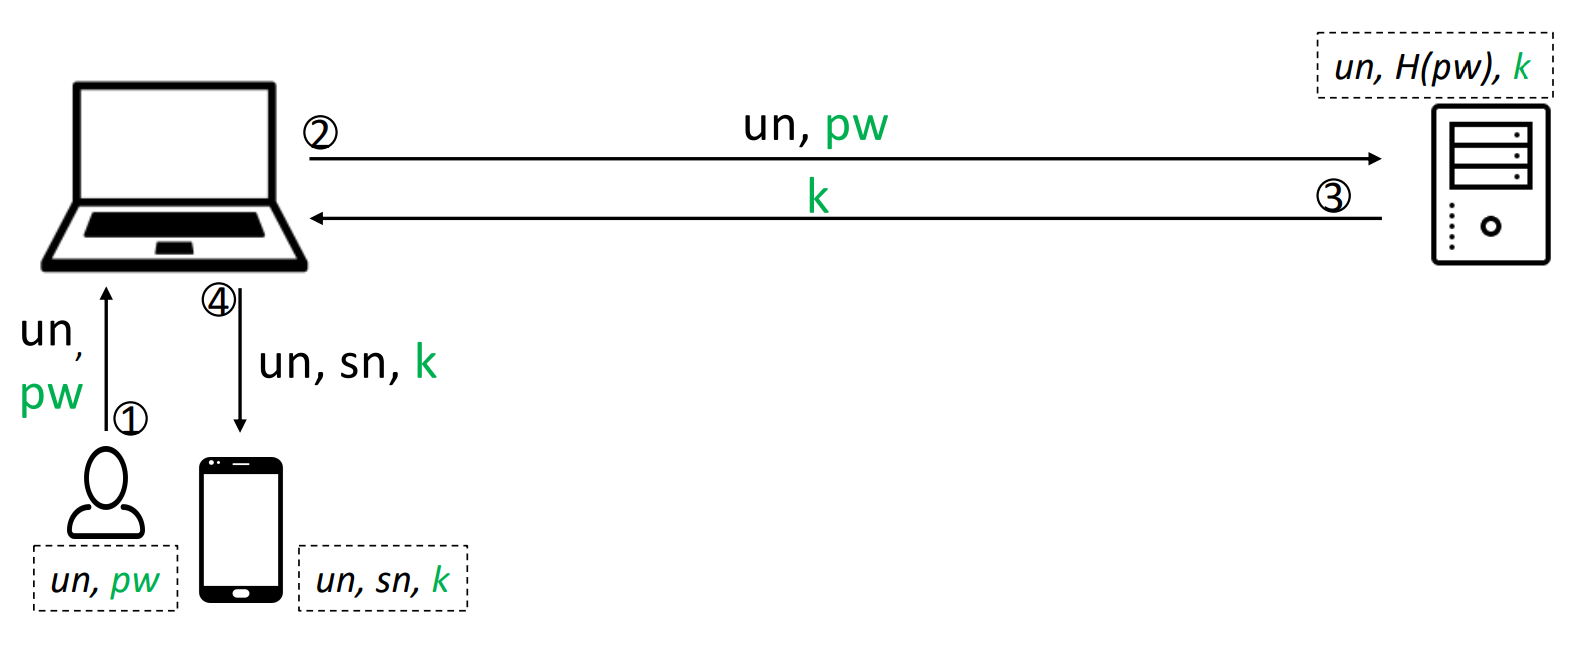
\includegraphics[scale=0.3]{registration.PNG}
    \caption{A diagram showing the interactions between the system
    components during the registration phase, as depicted by
    \cite{shirvanian2d2fa}.}
\end{figure}

During the registration phase, the parties involved in the 2D-2FA
protocol need to establish communication channels between them, and
share secret keys between the server and the device. 

First, a user would register their username and password with the
server. The server would pick a secret key for that user (generating it
from their password using HMAC). The secret then needs to be transferred
to the user's device (e.g., cell phone), which is typically done by
manually entering it into the device, or by scanning a QR code generated
by the server. This is so that the device will be able to generate PINs
later on in the 2D-2FA process. 

The server stores a hash of the user's password and secret key, and the
device stores only the secret key related to the user's account stored
on the server. The client (e.g., a web browser on a laptop that the user
uses to log in to the server) does not store any information during the
registration phase. 

\paragraph{Authentication Phase}

\begin{figure}
    \centering
    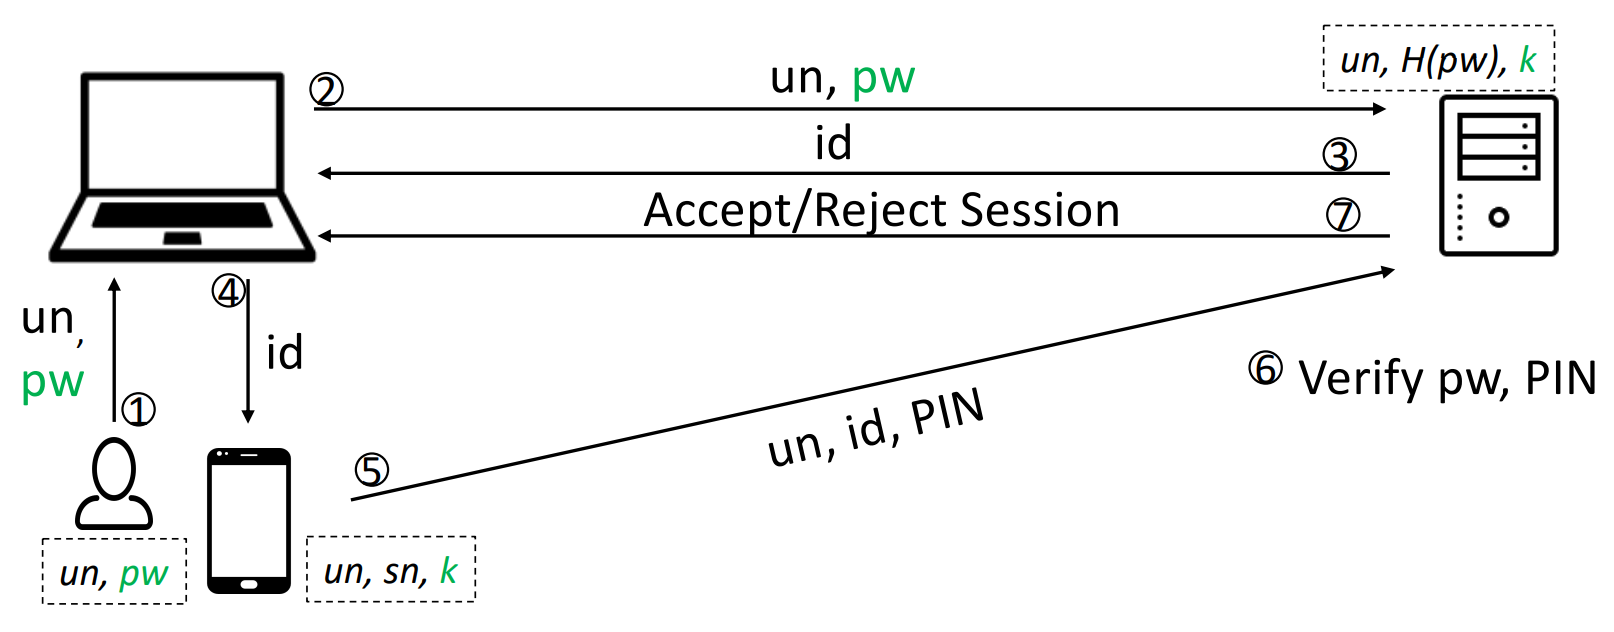
\includegraphics[scale=0.3]{auth.PNG}
    \caption{A diagram showing the interactions between the system
    components during the authentication phase, as depicted by
    \cite{shirvanian2d2fa}.}
\end{figure}

The authentication phase involves the interaction of the parties to
authenticate the user to the server securely. 

First, the user attempts to log in to the server from the client. The
user's login information (username and password) are used as the first
authentication factor. Next, the server displays a unique identifier to
the user through the client (the identifier can be implemented in a
variety of ways, either via QR code, a fourgram pattern as described in
section 6.1 of \cite{shirvanian2d2fa}, and so on). 

On the user's device, the user selects the server that they are logging
in to, and enters the identifier that was displayed to them on the
client. The device generates a PIN using the identifier, the current
time, and the user's secret key. The PIN and the identifier are sent to
the server.

When the server receives the PIN and the identifier, it authenticates
the user's session associated with the identifier, generating several
PINs to find one that matches with the time the PIN was generated on the
user's device. During this phase, the server keeps a temporary record of
all active sessions and identifiers.

%%%%%%%%%%%%%%%%%%%%%%%%%%%%%%%%%%%%%%%%%%%%%%%%%%%%%%%%%%%%
\subsection{Implementation}

Because of limited time and resources, we went with a software-only
implementation that can be accessed in the web browser. We used Python
because it is a language that we are familiar with, and it also offers a
diverse standard library, with built packages for networks and security.
To add a bare-bones user interface, we used Flask to make the
implementation of this interface easier. 

The system that we wrote includes implementations of the functions that
would run on the server and the device as described in
\cite{shirvanian2d2fa}. Specifically, we will discuss our
implementations for both the server and device, as well as go in-depth
into the minor differences between our implementation and the
implementation described in section 6 in \cite{shirvanian2d2fa}.

\paragraph{Device}

The device contains a list of servers, usernames used on those servers,
and keys for that server/username combination. In a full production
version, this would be generated in the registration phase; for our
proof-of-concept implementation, we simply included these in a text
file. The keys are loaded by a \texttt{load\_keylist} function that is
called once, and can be easily swapped out for a different function,
depending on how this information is stored in the final implementation.

The core of the device is the PIN generation. First, a time slice is
created by taking the current epoch time (in seconds) and dividing by a
fixed number, to get the current ``time slice''. This time slice is then
combined with an identifier using a bitwise exclusive or operation.
Finally, this combined value is hashed using HMAC, with the user's
secret key as the key and SHA256, to produce a PIN, which is sent along
with the username to the server.

Currently, the identifier is a six-digit number, as that is convenient
for implementing the device on a PC or laptop. This could easily be
changed out to a different identifier without any significant changes to
the existing code; the only addition would be code for inputting the
identifier.

Sending the PIN to the server is accomplished by a standard TCP message.
For the purposes of this proof-of-concept implementation, the device
uses a simple HTML interface for selecting the server/username and
inputting an identifier.



\paragraph{Server}
The server contains a list of \texttt{user:key} pairs, stored and
retrieved similarly to how the device handles its list of servers.

In a full deployment, the server-side code would be called by the login
portion of a server, likely either by importing the code or through
socket communication. For demonstration purposes, it currently uses a
simple HTML interface, where a user can input a name and receive both an
identifier and whether that name is authorized or not.

To handle identifiers, the server maintains a list mapping usernames to
identifiers. This list is initially empty. When asked for an identifier,
the server first checks this list, and if the username is there and the
identifier is not expired, it returns the found identifier. If not, it
generates a new identifier, saves the \texttt{user:identifier} pair to
the identifier list, and returns the identifier.

Upon receiving a username and PIN from a device, the server uses the key
and identifier it has saved for that user, and generates a series of
comparison PINs, using the same method the device used to generate its
own PIN. This series of comparison PINs is created using a range of time
slices (currently $\pm2$ time slices), in order to account for
differences in system clocks, transmission delays, etc. If any of these
comparison PINs match the PIN sent by the device, then the user is added
to the list of authorized users.

When the server is asked if a user is authenticated, it checks the
authenticated user list, and if the user is present and not expired,
then they are approved.

Both the identifier list and authenticated-user list include a
configurable expiration time for each item. The server ticks
periodically to check for expiration, and if the item is expired, it is
simply removed from the relevant list. Additionally, a ``minimum time''
can be specified on the server. When an identifier is requested, the
server checks how long it will be until the identifier will expire. If
this length of time is less than the specified minimum time, then the
old identifier is thrown out and a new identifier is generated, stored
in the identifiers list, and passed on to the user. This is done to
ensure the user has enough time to input the identifier before it
expires.

\paragraph{Implementation Differences}

The differences between our implementation and the implementation
described in section 6 of \cite{shirvanian2d2fa} were relatively minor,
especially for the authentication phase. Because our main motivations
for this project were to learn more about authentication security and
2FA, we were more interested in how the authentication phase was
accomplished, and thus spent less time on the implementation of the
registration phase. 

Because of this, our registration phase is already built-in to our
system by having a pre-defined set of users. Had we not done this, we
would have had to set up an account creation system, or some way to
create a new user and register the user with both the server and the
device. By having a pre-defined set of users, this meant that we could
have a user's secret keys already placed on the server and the device. 

We also used a 6-digit code for our identifier, instead of the fourgram
pattern or the QR code recommended by \cite{shirvanian2d2fa}. This made
our implementation easier, as we did not have to create a system to
display or interpret these patterns. In addition, had we used QR codes,
we would have had to find a way to implement the generation and scanning
of these codes, which we decided was outside the scope of the
project, and would likely have cost us too much time. 

Finally, we use the less secure TCP connections instead of TLS or SSL,
as recommended by \cite{shirvanian2d2fa}. We do not believe that this
compromises the security of our implementation, because these
connections are only for the channel between the device and the server.
This is satisfactory for our implementation because this channel is
expected to be a regular channel anyways (see the ``Channel Compromise''
in section 4). The TCP connections were also the easiest to implement
using Python's standard library \texttt{socket} API. 

%%%%%%%%%%%%%%%%%%%%%%%%%%%%%%%%%%%%%%%%%%%%%%%%%%%%%%%%%%%%
%%%%%%%%%%%%%%%%%%%%%%%%%%%%%%%%%%%%%%%%%%%%%%%%%%%%%%%%%%%%
\section{Security Analysis}

There are several possible avenues of attack to the 2D-2FA system that
are proposed in \cite{shirvanian2d2fa}. In this section, we will go over
each attack vector and analyze how the system protects against these
attacks, as well as explaining how our implementation prevents these
attacks. 

\paragraph{Client Compromise}
In this attack, an attacker would have compromised the client that the
user uses to log into the server, and thus gain access to the user's
password. Assuming the device is not also compromised, the user's
account is still secure. 

This attack is prevented because once an attacker logs in using the
user's password, they will receive an identifier generated by the
server. But, without access to the user's secret key, the attacker has
no means of computing a PIN that corresponds to the identifier, and
thus no means of providing a valid PIN to the server. Additionally,
without access to the user's device, the attacker has no way to generate
a valid PIN without guessing the user's secret key, which would not be
feasible. 

% In our implementation, 

\paragraph{Device Compromise}
In this attack, an attacker would have compromised the user's device,
and as such they have full control over the device. In this attack
vector, we assume that the attacker has access to the secret information
stored on the device. This allows the attacker to generate any PIN, for
any identifier.

This attack is prevented because for the attacker to gain access to the
user's account, the attacker still needs to know the user's password to
log in on the client. If the user has chosen a secure password that can
not easily be guessed, the attacker must guess the user's password to
gain access to their account, which would not be feasible. 

% In our implementation, 

\paragraph{Channel Compromise}
In this attack, an attacker has control over the channels connecting the
parties (the client, device, and server) in the system. Specifically,
there are three main channels in the 2D-2FA system. The channel between
the client and the server is secure, the channel between the client and
the device is through the user, and the channel between the device and
the server is a regular channel. In this attack vector, the attacker
could either listen to the channels (eavesdrop), or they could modify or
block the network traffic. 

This attack is prevented because the time slice is not exclusively used
to generate the PIN. Because of the fact that each identifier is unique,
if a PIN that is sent on the channel corresponds to the time slice that
the attacker needs, it will not correspond to the identifier that the
attacker needs. This renders the copying of data from the device-server
channel useless. 

% In our implementation, 

\paragraph{User Negligence}
In this attack, a user is simply negligent, and inadvertently grants
access to an attacker. 

This attack is prevented because, a user would only accidentally approve
an attacker's session when the user enters the identifier that is
displayed to the attacker, rather than the identifier that is displayed
to the user. Depending on the type of identifier used, the possibility
of this occurring is very low.

In our implementation, we used a 6-digit identifier, which means that if
an attacker has logged in and is presented with an identifier, the user
has a one-in-a-million chance (0.0001\%) of approving that attacker's
session. 

\paragraph{Attacks on Third Parties}
In other MFA systems, third party entities are introduced, such as a MFA
service provider. The system owner would need to trust these service
providers, as well as study the security of the services that they
provide to be comfortable with the security of their services. Attackers
can target these third parties, as well as the channels connecting the
third party services to the main system, which increases the complexity
of the security analysis of the system. 

Because 2D-2FA does not use any third party systems, this decreases the
complexity of the security analysis, and thus reduces the surface of
attack into the system. Additionally, 2D-2FA only uses well-established
and well-studied technologies (HMAC, SSL/TLS, random number generation,
etc.), further reducing attack vectors.

In our implementation, we use the well-established technologies
mentioned in and used by \cite{shirvanian2d2fa}, the only variation
being that we use TCP connections instead of using TLS.

%%%%%%%%%%%%%%%%%%%%%%%%%%%%%%%%%%%%%%%%%%%%%%%%%%%%%%%%%%%%
%%%%%%%%%%%%%%%%%%%%%%%%%%%%%%%%%%%%%%%%%%%%%%%%%%%%%%%%%%%%
\section{Conclusion}

We created a proof of concept implementation of the 2D-2FA system,
finding that it was easy to understand, build, and use. While we did not
attempt to attack our system, we found the security analysis in
\cite{shirvanian2d2fa} to be clear, thorough, and reasonable. Moreover,
we did find that the design goals laid out in section 3.3.2 of
\cite{shirvanian2d2fa} were accomplished during our implementation. It
was relatively easy to implement our system, easy to use, and only made
use of the Python standard library (except Flask, which was used for the
simple web interface). 

%%%%%%%%%%%%%%%%%%%%%%%%%%%%%%%%%%%%%%%%%%%%%%%%%%%%%%%%%%%%
\subsection{Complications}

There were relatively few complications that arose during our project,
all of which we were able to overcome. The first arose when we were
trying to figure out the socket communications in the Python
environment. However, after reading some documentation and getting a
better understanding of the Python standard library socket API, we were
able to successfully communicate between the device and the server. 

Finally, because of the limitations of what information can be passed
between the server and the device, we had to use two threads in the
server to get everything working correctly. These threads did the
following, respectively: 
\begin{enumerate}
    \item listen for connections from the device, verify the PIN that
    was sent from the device, add a user to the ``authorized'' list, and
    check for expired entries on the identifier list and authorized
    list;
    \item run the Flask app, listen for users logging in, generate the
    identifier, display the identifier to the user, and check if a user
    is authorized (on the authorized list). 
\end{enumerate}
However, once we figured out that the server code needed multiple threads to
function as desired in our implementation, it was relatively light work
to add the multithreaded functionality. 

%%%%%%%%%%%%%%%%%%%%%%%%%%%%%%%%%%%%%%%%%%%%%%%%%%%%%%%%%%%%
\subsection{Lessons}

The important lessons that we have learned include project planning,
collaboration skills, and iterative development. While we had prior
experience in all of these areas from previous projects, this project
helped ingrain these principles into how we worked, altogether adding to
a better workflow and increased productivity. 

For the project planning, we had thoroughly read through the
implementation section in \cite{shirvanian2d2fa}. From this, we 
broke down each element of the implementation into smaller chunks that
were easier to tackle and implement. This allowed us to develop one
module at a time, and ensure that module was functioning in the desired
way before continuing to the next module. 

In terms of collaboration, we have weekly meetings where we discuss what
we have accomplished in the past week, and what we plan on completing
for the next week. During the week, we update each other with our
progress, as well as asking questions or seeing if we have suggestions
for each other. 

With regard to iterative development, this goes hand in hand with our
project planning. Because we have broken down the problem into
bite-sized chunks, we can iteratively implement these small portions,
easily adding features and functionality to them as we progress, and
iteratively changing them or modifying them when we encounter the need
to do so.

%%%%%%%%%%%%%%%%%%%%%%%%%%%%%%%%%%%%%%%%%%%%%%%%%%%%%%%%%%%%
\subsection{Recommendations}

While the study completed in \cite{shirvanian2d2fa} found that 75\% of
users preferred 2D-2FA over the more commonly know PIN-2FA, we believe
that 2D-2FA could be better used in tandem with another 2FA method.
There are multiple 2FA methods we found, most notably Sound-Proof
\cite{soundProof} and Typing-Proof \cite{liuTypingProof}. For the
purposes of brevity, we will focus on how 2D-2FA can be used with
Typing-Proof. 

Typing-Proof, introduced by Liu, Li, and Deng, uses a registered phone
to listen to the user's keystrokes when they type a random code
presented to them during login. The time between the keystrokes is also
recorded by the server, and is compared with the recording taken by the
user's device. When the timing between the keystrokes recorded by the
device and by the server match, the user is successfully authenticated. 

The advantages that Typing-Proof brings to the table is decreased login
time, as well as less interaction between the user and their personal
device, which can be cumbersome and annoying, thus increasing usability
\cite{liuTypingProof}. In fact, the system usability scale (SUS) score
of Typing-Proof is 81.7, whereas the SUS of 2D-2FA is 75. This is likely
because 2D-2FA still requires the user to interact with their device by
entering the identifier. Note, however, that no study comparing the two
2FA methods has been conducted.  

We believe that Typing-Proof is a strong alternative to 2D-2FA, and it
could be used in tandem with 2D-2FA. In such a scheme, a user might
log in normally, with their device listening to their keystrokes. If
they are in a loud or busy environment, such as a caf\'e,
\cite{liuTypingProof} found that users are less likely to user
Typing-Proof. In this case, it would be convenient to use 2D-2FA as an
alternative. Additionally, Typing-Proof has a measured false acceptance
rate of about 0.015, and during cases where the device is unsure about
the validity of the keystrokes it heard, it could use 2D-2FA instead.

% Possibly add to this with typing proof \cite{liuTypingProof}

%%%%%%%%%%%%%%%%%%%%%%%%%%%%%%%%%%%%%%%%%%%%%%%%%%%%%%%%%%%%
%%%%%%%%%%%%%%%%%%%%%%%%%%%%%%%%%%%%%%%%%%%%%%%%%%%%%%%%%%%%
\bibliographystyle{ieeetr}
\bibliography{ref}

\appendix
\section{Description of Developed Software}

Descriptions of the software we developed can be found in the function
description comments and the file description comments for the code we
wrote. The program files are in the /src directory of the
repository. 

\end{document}
